\documentclass[tikz,border=8pt]{standalone}
\begin{document}
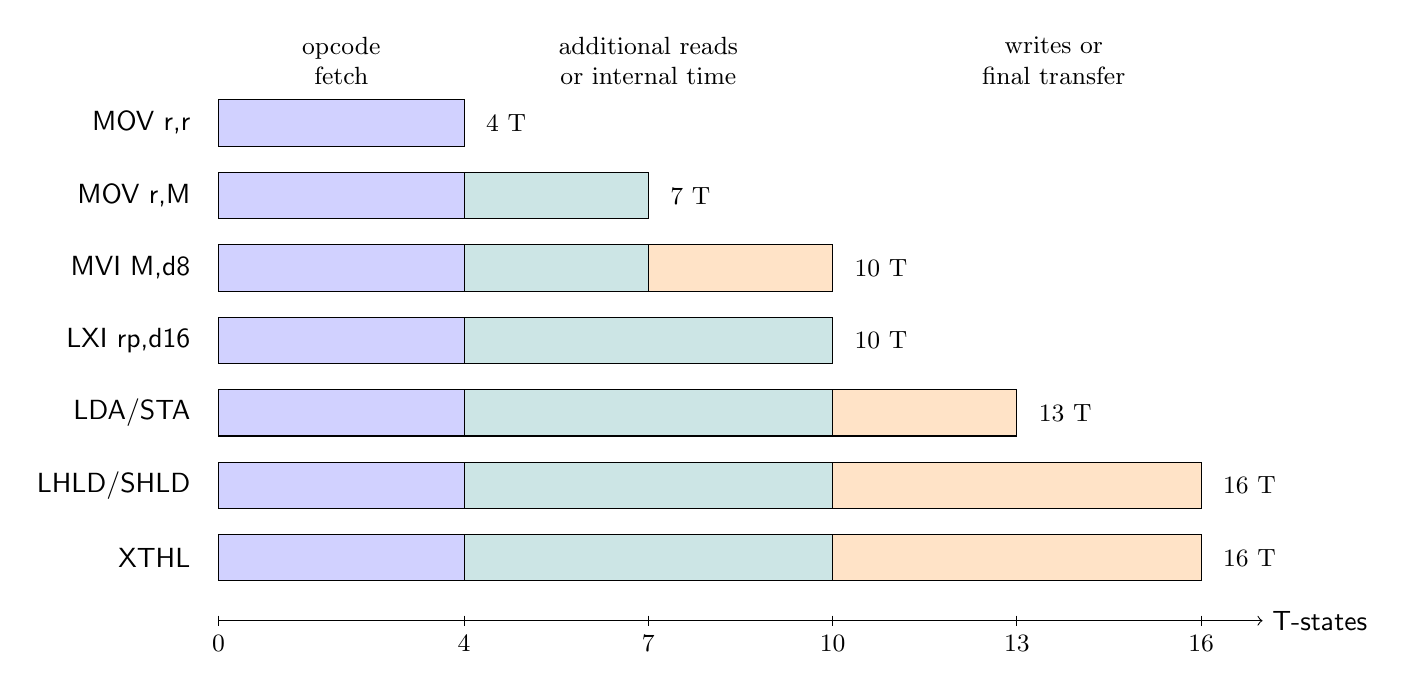
\begin{tikzpicture}[font=\sffamily,x=.78cm,y=.92cm]
\def\row#1#2#3#4#5{\node[anchor=east] at (-.3,#1+.32){#2};\draw[fill=blue!18] (0,#1) rectangle (#3,#1+.64);\draw[fill=teal!20] (#3,#1) rectangle (#4,#1+.64);\draw[fill=orange!22] (#4,#1) rectangle (#5,#1+.64);\node[anchor=west,font=\small] at (#5+.2,#1+.32){#5 T};}
\row{6}{MOV r,r}{4}{4}{4}
\row{5}{MOV r,M}{4}{7}{7}
\row{4}{MVI M,d8}{4}{7}{10}
\row{3}{LXI rp,d16}{4}{10}{10}
\row{2}{LDA/STA}{4}{10}{13}
\row{1}{LHLD/SHLD}{4}{10}{16}
\row{0}{XTHL}{4}{10}{16}
\node[font=\small,align=center] at (2,7.18){opcode\\fetch};\node[font=\small,align=center] at (7,7.18){additional reads\\or internal time};\node[font=\small,align=center] at (13.6,7.18){writes or\\final transfer};
\draw[->] (0,-.55)--(17,-.55) node[right]{T-states};
\foreach \x in {0,4,7,10,13,16}{\draw (\x,-.48)--(\x,-.62) node[below,font=\small]{\x};}
\end{tikzpicture}
\end{document}
